\chapter[Capítulo 3. Background en algoritmos de árboles de decisión]{Background en algoritmos de árboles de decisión}

\section{Fundamentos de árboles de decisión}

 Los \textbf{árboles de decisión} \cite{ref3} son un tipo de algoritmos de aprendizaje supervisado (tanto para clasificación como para regresión) utilizado en diversos ámbitos como la inteligencia artificial, las finanzas, el marketing, etc. \\ Dado un conjunto de datos se fabrican diagramas de construcciones lógicas en forma de ramificaciones de árboles, muy similares a los sistemas de predicción basados en reglas, que sirven para representar y categorizar una serie de condiciones que ocurren de forma sucesiva, para la resolución de un problema.
 
 Adentrándonos en los aspectos más técnicos de este tipo de modelos de predicción, cabe destacar que las variables de entrada y de salida pueden ser tanto categóricas como continuas y que divide el espacio de los predictores (variables independientes) en regiones distintas y no superpuestas, tal como veremos en la siguiente figura.
 
 \begin{figure}[H]
 	\centering
 	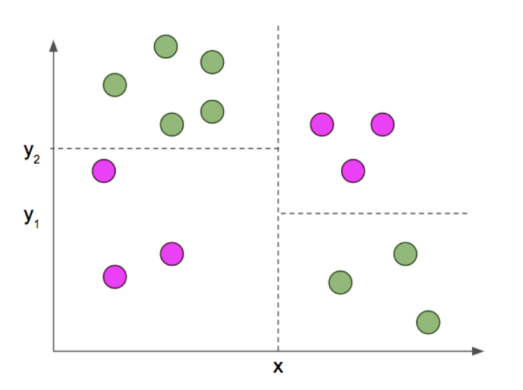
\includegraphics[width=0.7\textwidth]{imagenes/ejemploArboles} 
 	\caption{Ejemplo de árbol de decisión \cite{ref4}}
 \end{figure}
 
 Estas divisiones se realizan creando sobre la población (el conjunto de datos) subconjuntos lo más homogéneos posible entre las muestras que componen un grupo y lo más heterogéneo posible entre los distintos subconjuntos.\\
 Para la efectuación de esta separación, el algoritmo se basa en las variables de entrada más significativas, es decir, las que mejor separan las muestras.
 
 A continuación podemos observar las diferentes partes de un árbol de decisión.
 
  \begin{figure}[H]
 	\centering
 	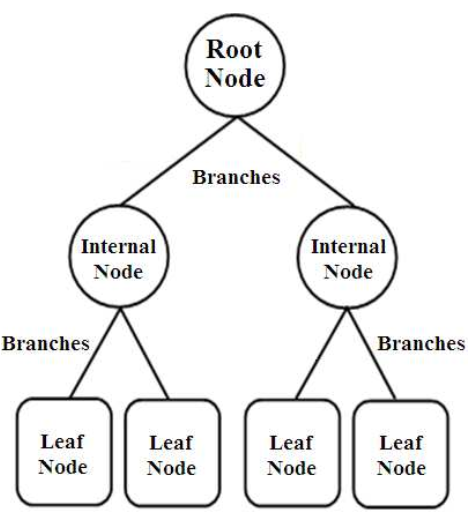
\includegraphics[width=0.5\textwidth]{imagenes/ejemploArbol} 
 	\caption{Partes de un árbol de decisión \cite{ref5}}
 \end{figure}

\subsection{Terminología:}
\begin{itemize}
	\item \textbf{Nodo raíz}: Es el primero de los nodos del árbol y forma la población completa.
	\item \textbf{Ramificación}: Son las ramas que conectan todos los nodos del árbol por donde pasan las muestras para ser clasificadas.
	\item \textbf{Nodo de decisión}: Son aquellos donde las muestras se evaluan para decidir por qué rama continuar el camino hacia la solución.
	\item \textbf{Nodo terminal/hoja}: Estos son los nodos solución, una vez la muestra llega a este tipo de nodo, el proceso de evaluación de esta ya ha finalizado, por lo que habrá sido clasificada en alguno de los grupos categóricos existentes.
	\item \textbf{Poda}: Consiste en cortar u obviar una rama del árbol en la creación de un árbol, basándonos en cierta propiedad escogida, para evitar el recorrido del árbol completo y ahorrar de esta forma costos computacionales, así como para hacer frente al sobreajuste.
	\item \textbf{Rama/subárbol}: Es el conjunto de nodos y ramas completo que queda estrictamente por debajo de un nodo escogido del árbol total.
	\item \textbf{Nodos padre e hijo}: Dado un nodo del árbol, sus nodos hijo son todos aquellos que quedan conectados directamente a él únicamente en el nivel inferior siguiente. De esta forma, esos nodos hijo, comparten ese mismo padre.
\end{itemize}


\subsection{¿Regresión o clasificación?: similitudes y diferencias.}

\subsubsection{Similitudes}

Ya sabemos, por ejemplo, que un árbol de decisión divide el espacio de los predictores en regiones no solapadas mediante el uso de los predictores más significativos.

Los árboles de decisión actúan bajo la llamada \textbf{separación binaria recursiva}, basada en un método greedy el cual decidirá en cada momento cuál será la mejor separación en el instante actual para encontrar el mejor árbol. El término 'binaria' hace alusión al tipo de división acaecido en cada nodo, es decir, que cada nodo divide en dos el espacio de los predictores. El término 'recursiva' se refiere a que el algoritmo realiza este proceso de forma reiterada hasta llegar a un criterio de parada predefinido.

Este proceso nos conduce a la generación de un árbol completo si no hacemos uso de criterios de parada, lo que nos lleva de forma directa al problema del sobreajuste, obteniendo un modelo de una pésima calidad a la hora de evaluar nuevos datos. Por esto mismo es necesario difinir criterios de parada que realicen podas sobre el árbol para generar modelos lo suficientemente genéricos que eviten ese overfitting.

\subsubsection{Diferencias}

Las diferencias entre ambos modelos son bastante evidentes: para conjuntos de datos donde se utiliza una variable dependiente continua, utilizamos árboles de regresión, mientras que cuando la variable dependiente es categórica, usamos árboles de clasificación.\\
Dado esto, el \textbf{valor de los nodos hoja} no pueden ser calculados de la misma forma para ambas técnicas, por lo que, en \textbf{árboles de regresión}, utilizamos la \textbf{media} del valor de salida de las muestras que caen en dicho nodo hoja, mientras que en \textbf{árboles de clasificación} utilizamos la \textbf{moda} para asignar un valor de salida a nuevas muestras.

\subsection{Ventajas e inconvenientes de los árboles de decisión}

\subsubsection{Ventajas}

\begin{itemize}
	\item Fáciles de comprender a la hora de interpretar los resultados.
	\item El tipo de dato utilizado no es una limitación.
	\item Es un método no paramétrico, es decir, en el que no es necesario hacer suposiciones sobre el espacio de distribución y la estructura del clasificador.
	\item Resulta útil a la hora de detectar la relevancia de los predictores aún habiendo una gran cantidad de estos.
	\item No son influidos por outliers ni valores perdidos (hasta cierto punto), por lo que requieren una menor limpieza de datos en comparación con otros métodos.
\end{itemize}

\subsubsection{Inconvenientes}

\begin{itemize}
	\item Producen sobreajuste, por lo que hay que tener cuidado con ello mediante el uso de restricciones y la aplicación de poda.
	\item A la hora de trabajar con variables continuas, el árbol de decisión pierde información en el momento en el que categoriza dichas variables para la generación del árbol.
	\item No son del todo competentes con los mejores algoritmos de aprendizaje supervisado en cuanto a precisión en la predicción, es decir, no resultan ser tan efectivos ensambladores o SVM por ejemplo.
	\item Son sensibles al ruido en los datos, ya que este puede modificar de forma significativa la estructura del árbol.
\end{itemize}

\subsection{Creación del árbol}

Como ya sabemos, un árbol comienza desde un nodo raíz donde se encuentra clasificada toda la población y, conforme vamos profundizando por las ramas inferiores, vamos obteniendo subconjuntos cada vez más y más homogéneos con respecto a la variable de salida.

Para hacer posible esto necesitamos que nuestro modelo tome, por cada nodo, una decisión de separación de los datos basada en la ganancia de pureza (esa homogeneidad en los subconjuntos) al utilizar uno u otro predictor en cada uno de los nodos de decisión para crear esas particiones del espacio sucesivas.\\
Es decir, para cada nodo, se evalúa mediante unos medidores de pureza, cual es el predictor o característica del conjunto de datos en dicho instante que separa de mejor forma los datos que tenemos en ese momento con respecto a la variable de salida. Se escogerá en cada nivel, el predictor que mayor pureza ofrezca al árbol de decisión.

De esta forma vamos construyendo de manera progresiva ramas y más ramas del árbol haciendo uso de una técnica greedy de selección de característica a evaluar en cada nivel del árbol para la toma de decisión a la hora de generar nuevos nodos hijos.

\subsubsection{¿Cómo medimos esa ganancia de homogeneidad?}

Para los\textbf{ árboles de regresión} sabemos que el objetivo de cada decisión del árbol en la creación de nuevas separaciones es minimizar la función RSS (\textbf{Residual Sum of Squares}), una medida de error usada también en la regresión lineal. Es por ello que en cada nodo se escogerá una forma de particionar los datos mediante el uso de un predictor u otro, atendiendo a cuál minimiza en mayor medida dicha fórmula.

\begin{figure}[H]
	\centering
	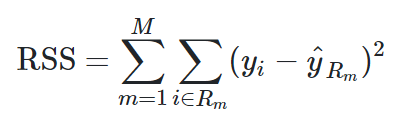
\includegraphics[width=0.5\textwidth]{imagenes/rss} 
	\caption{Recursive Binary Splitting in regression trees \cite{ref6}}
\end{figure}

Como el problema que nos concierne en este caso es el de \textbf{árboles de clasificación}, no entraremos en más detalles acerca de esta fórmula, ya que RSS no puede ser utilizado como criterio de separación binaria en este tipo de árboles.

Una aproximación natural a RSS es el '\textbf{ratio de error en la clasificación}', basado simplemente en la fracción de las observaciones de training en dicha región que no pertenecen a la clase más común de esta. Se calcula de la siguiente forma:

\begin{figure}[H]
	\centering
	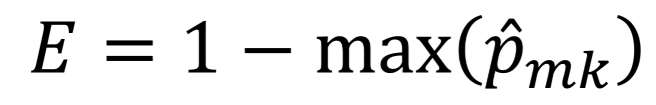
\includegraphics[width=0.5\textwidth]{imagenes/cer} 
	\caption{Recursive Binary Splitting in classification trees (classification error rate) \cite{ref7}}
\end{figure}

Donde $\widehat{P}$mk es la proporción $\widehat{P}$ de las observaciones de train de la región \textbf{m} que pertenecen a la clase \textbf{k}. Por tanto, el máximo de $\widehat{P}$mk hace alusión a la proporción máxima de elementos de train que siguen la moda en dicha partición.\\
Por desgracia esta medida de error no es lo suficientemente sensible conforme el árbol crece, por lo que es preferible el uso de otras medidas como el índice Gini y la Entropía.

Ya sabemos que buscamos nodos con una distribución de clase lo más homogénea posible. Con el fin de medir esa pureza en cada nodo, podremos utilizar los siguientes métodos ya mencionados:
\begin{itemize}
	\item \textbf{Índice GINI}: nos indica como de pura es una región del espacio. En este caso la pureza la definimos como la proporción de items de la región que pertenecen a una misma clase. Si la región contiene un índice
	alto de pureza, entonces el índice Gini será bajo (muy próximo a 0), siguiendo la siguiente fórmula:
	\begin{figure}[H]
		\centering
		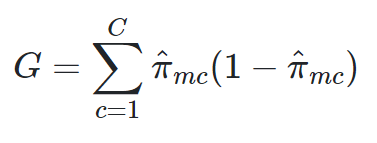
\includegraphics[width=0.5\textwidth]{imagenes/gini} 
		\caption{Recursive Binary Splitting in classification trees (gini) \cite{ref8}}
	\end{figure}
	Donde $\widehat{\pi}$mc nos indica la proporción \textbf{$\widehat{\pi}$} de items pertenecientes a la misma clase \textbf{c} en la región/nodo \textbf{m}.
	\item \textbf{Entropía (E-score)}: Se encarga también de la medida de homogeneidad de un nodo. En este caso, los resultados obtenidos al aplicar la siguiente fórmula a cada nodo para observar el nivel de entropía, quedan más visibles con respecto a la medida Gini (es decir, se ve de forma más clara el nivel de homogeneidad de un nodo). Una entropía = 0 significa homogeneidad total, una entropia = 1 significa homogeneidad nula.
	\begin{figure}[H]
		\centering
		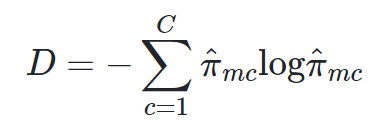
\includegraphics[width=0.5\textwidth]{imagenes/entropia} 
		\caption{Recursive Binary Splitting in classification trees (entropia) \cite{ref8}}
	\end{figure}
\end{itemize}

\subsubsection{¿Cómo evitamos el overfitting?}

Una vez hemos escogido nuestra estrategia de creación del árbol, necesitamos indicarle al algoritmo cuándo ha de terminar de construirlo el uso de restricciones (prepruning) y su posterior poda (postpruning) para evitar de esta forma un sobreajuste a los datos.\\

\textbf{Prepruning: establecimiento de parámetros}
\begin{itemize}
	\item Definir un número de observaciones mínimo sobre un nodo para que sea considerada una ramificación sobre él.
	\item Definir un número mínimo de observaciones sobre un nodo hoja.
	\item Establecer una profundidad vertical máxima para el árbol.
	\item Limitar el número máximo de nodos hoja.
	\item Parar si la expansión del nodo actual no mejora la medida de pureza utilizada actual.
\end{itemize}

\textbf{Proceso de Postpruning}:
\begin{enumerate}
	\item Crear un árbol muy grande con o sin restricciones de prepruning.
	\item Recorrer el árbol de abajo hacia arriba para ir cortando las hojas que nos dan ganancias negativas.
\end{enumerate}

De esta forma podemos mantener ramas que, sin el proceso de postpruning podrían haber sido recortadas, pero que nos llevan a soluciones mejores que las que se ofrecen si este proceso por culpa del uso de la técnica greedy.


\section{Hoeffding Trees y otros algoritmos de data streaming}

Como ya sabemos, los algoritmos dedicados al data streaming han de seguir los siguientes requisitos:
\begin{itemize}
	\item Procesar una muestra en cada momento y hacerlo tan solo una vez.
	\item Usar una cantidad de memoria limitada.
	\item Trabajar en un tiempo limitado.
	\item Estar listo para la predicción en cualquier momento.
\end{itemize}

Además, nuestro algoritmo ha de estar dotado de técnicas de detección de cambios en la distribución de los datos para evitar la disminución de la precisión en la predicción cuando esto suceda.

\subsection{Hoeffding tree (VFDT)}

Un árbol de Hoeffding es un algoritmo de inducción de árbol de decisión incremental capaz de aprender de flujos de datos masivos, suponiendo que la distribución que genera ejemplos es estacionaria, es decir, que no cambia con el tiempo. Los árboles Hoeffding explotan el hecho de que una pequeña muestra a menudo puede ser suficiente para elegir un atributo de división óptimo. Esta idea está respaldada matemáticamente por el Hoeffding bound, que cuantifica el número de observaciones (en nuestro caso, ejemplos) necesarias para estimar algunas estadísticas dentro de una precisión prescrita (en nuestro caso, la bondad de un atributo). \cite{ref9}

Algunas de las técnicas de clasificación para data streaming tienen los siguientes \textbf{problemas}:
\begin{itemize}
	\item Son altamente sensibles a la demanda de ejemplos.
	\item Carecen de alta eficiencia, siendo en algunos casos más lentos que un algoritmo batch.
\end{itemize}

Ante estos problemas se plantea\textbf{ Hoeffding-tree} ya que:
\begin{itemize}
	\item El aprendizaje de un Hoeffding-tree toma un tiempo constante en cada nuevo ejemplo, lo que lo hace adecuado para el aprendizaje de flujos de datos.
	\item Los árboles resultantes son similares a los creados con un batch learner convencional.
\end{itemize}

\subsubsection{Hoeffding bound.}

Hulten y Domingos presentan un método general para aprender de bases de datos grandes y arbitrarias.
Este método consiste en derivar un límite superior para la pérdida del learner en función del número de ejemplos usados en cada paso del algoritmo. De esta forma, se minimiza el número de ejemplos requeridos en cada paso del algoritmo, a la vez que se garantiza que el modelo obtenido no difiere de forma significante de aquel que se obtendría con todos los datos. Esta metodologia de datos se ha aplicado de forma exitosa en k-means, clustering jerárquico de variables, árboles de decision, etc.

Con el fin de cumplir con los requisitos establecidos al principio de este apartado para el tratamiento de flujos de datos, los autores proponen la cota Hoeffding para ser capaces de decidir la cantidad de instancias necesarias a evaluar para alcanzar un cierto nivel de confianza a partir del cual sabemos que no es necesario evaluar más ejemplos para seleccionar un atributo mediante el cual realizar la partición del árbol en el nodo actual.\\
Es decir, una vez alcanzada la cota de Hoeffding, el atributo que seleccionemos para el particionamiento del espacio de predictores, sera el mismo que seleccionariamos si analizásemos una infinidad de ejemplos con el clasificador (evidentemente, con cierto nivel de confianza).

La idea básica consiste en usar un conjunto pequeño de ejemplos para seleccionar el test de divisón para colocar en un nodo del árbol de decisión.
Si tras ver un conjunto de ejemplos, la diferencia en resultados entre ambos test de división no satisface un test estadístico (Hoeffding bound), entonces VFDT procede a examinar más ejemplos.

En VFDT se aprende un árbol de decisión de forma recursiva reemplazando hojas por nodos de decisión. Cada hoja almacena las estadísticas necesarias sobre los valores de los
atributos. Dichas estadísticas necesarias son aquellas que se necesitan por una función de evaluación heurística que realiza el cálculo del resultado de los test de división 
basada en el valor de los atributos.
Cuando hay un ejemplo disponible, atraviesa el árbol desde la raíz hasta una hoja evaluando el atributo requerido en cada nodo y siguiendo la rama correspondiente al valor
del atributo en el ejemplo.
Cuando el ejemplo llega a una hoja, la estadística de las hojas por las que ha pasado han sido actualizadas.
Entonces cada condición basada en los valores de los atributos ha sido evaluada.

El nuevo nodo de decisión tendrá tantos descendientes como el número de posibles valores tenga el atributo escogido (por lo que el árbol no es necesariamente binario).
Los nodos de decisión tan solo contienen la información sobre el test de división instalado en ellos.

\textbf{Problema}: VFDT no incluye soporte para el concept-drift por lo que, ante cambios en la distribución de los datos, los resultados del algoritmo pueden ser malos.

\textbf{Cálculo de la cota:}

Teniendo n variables independientes $r_{1}...r_{n}$ con un rango R y una media $\bar{r}$, el Hoeffding bound afirma con una probabilidad 1-$\delta$ que la media real es al menos $\bar{r}$-$\epsilon$ donde:
\begin{figure}[H]
	\centering
	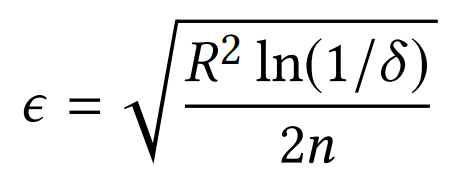
\includegraphics[width=0.3\textwidth]{imagenes/hoeffdingbound} 
	\caption{Cálculo del límite de Hoeffding \cite{ref10}}
\end{figure}

Sabiendo que $\delta$ es la tolerancia al fallo a la hora de escoger un atributo en un nodo dado.

\subsection{Otros algoritmos de data streaming}

Muchas bases de datos grandes presentan cambios en la distribución de los datos conforme avanza la generación de estos, es decir, posee un cambio de concepto en el tiempo, un \textbf{concept drift}. El hecho de que un algoritmo de flujos de datos no esté preparado para esos efectos cambiantes puede producir un empeoramiento de los resultados predictivos con el paso del tiempo, por lo que conviene tenerlo en cuenta a la hora de implementar esta clase de algoritmos.

Ante este problema, surgen técnicas como el uso de una \textbf{ventana deslizante} que tenga en cuenta los X ejemplos más recientes para asegurarnos de aprender siempre un modelo que tenga en cuenta el concepto actual se los datos, olvidando conceptos anteriores. Ante esta situación, ha de tenerse cuidado de escoger un valor adecuado de X, ya que ha de ser lo suficientemente grande como para tener un número suficiente de ejemplos con los que aprender el modelo y lo suficientemente pequeño como para abarcar un solo concepto de los datos.

\subsubsection{CVFDT}

Un algoritmo que utiliza este concepto de ventana deslizante es el llamado\textbf{ Concept-adapting Very Fast Decision Tree (CVFDT)} que, evidentemente, contiene además las características del VFDT. A continuación la explicación de su funcionamiento\cite{ref12}:

\begin{figure}[H]
	\centering
	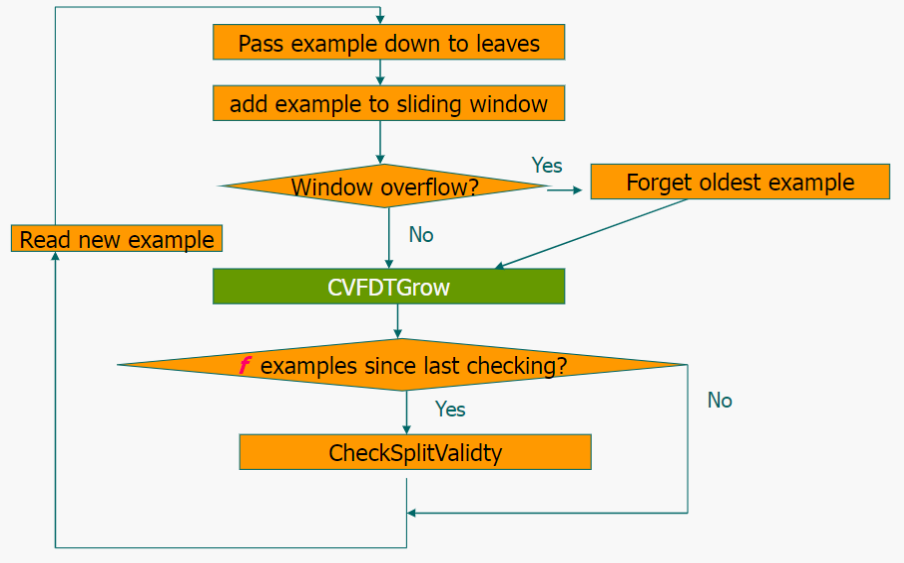
\includegraphics[width=1\textwidth]{imagenes/cvfdt} 
	\caption{Ciclo CVFDT \cite{ref11}}
\end{figure}

\begin{enumerate}
	\item Entra un nuevo ejemplo al ciclo.
	\item Se añade a la ventana deslizante.
	\item Se comprueba si se excede la cantidad de ejemplos necesarios en dicho nodo para poder decidir el atributo apropiado para la división de los nodos hijos. En caso de excederse dicho tamaño de ventana, se elimina el ejemplo más antiguo.
	\item CVFDTGrow: Se incrementan las estadísticas de cada uno de los nodos por los que pasa el ejemplo tanto en el árbol principal como en los subárboles. Si se ha alcanzado la cantidad suficiente de elementos analizados como para expandir un nodo hoja, escogemos el mejor de los atributos para expandir y se procede a ello.
	\item CheckSplitValidity: Comprueba si comenzar un árbol alternativo o no basado en el atributo que mejor realiza la división en cada uno de los nodos. Se realiza una comprobación de las estadísticas de cada nodo observando si se produce un cambio de concepto con el nuevo ejemplo, en cuyo caso es posible que el atributo escogido anteriormente en dicho nodo posea una ganancia menor que otro, por lo que el algoritmo creará un subárbol alternativo cuya raíz será ese atributo que tenga mejor gain que el actual en dicho nodo.
\end{enumerate}

Cada uno de los nodos de decisión ha de tener las estadísticas suficientes para poder olvidar información en caso de que se produzca un cambio de concepto. Para ello, cada uno de los nodos posee un ID monotónicamente incremental que permite al algoritmo validar las decisiones previamente tomadas y realizar el olvido de información inútil en los cambios de concepto. Cuando un ejemplo antiguo es eliminado de la ventana, se recorre el árbol para decrementar las estadísticas por cada uno de los ID de los nodos por los que ha pasado.


\subsubsection{HATT}

Otro algoritmo que implementa una solución más eficiente a la presentada por Hoeffding tree es el \textbf{Hoeffding Anytime Tree} \cite{ref10}, el cual asegura conseguir mejores resultados explotando la información conforme le llega al modelo en lugar de esperar a traspasar el Hoeffding bound y, realizando correciones sobre estas decisiones de elección de atributo para la división siempre que sea necesario.
Por tanto, en cuanto se detecte una división útil en cualquiera de las hojas del árbol, se realizará de forma inmediata y esta, será reemplazada tan pronto como otra alternativa mejor sea identificada.

Además de esto, algunos experimentos muestran que el algoritmo, aún no habiendo sido tratado para ello, muestra algunas características de tratamiento de concept drift.

\subsubsection{Option trees}

Con el objetivo de introducir a Hoeffding tree mayor estabilidad y romper la barrera que posse VFDT para mirar hacia adelante, surje Option trees\cite{ref13}.\\
Consiste en una estructura que representa a múltiples árboles en lugar de a uno solo como hace VFDT. Una instancia nueva puede bajar por varios caminos del árbol contribuyendo de diferentes maneras en diferentes opciones. La clase de un ejemplo de test se determina por un comité(mayoría de voto o pesos) hecho por las predicciones de todas los nodos hoja alcanzados. El concepto es crear múltiples opciones pero de la misma forma que lo hace Hoeffding tree.\\
Esta nueva representación de un árbol difiere únicamente de la representación hecha para VFDT en que contienen unos nodos llamados \textbf{nodos opción} que se encargarán de evaluar a los ejemplos que pasen por ellos mediante múltiples tests para determinar por qué ramas dejarle pasar.\\
En este nuevo método, un ejemplo que entra al árbol puede influir en varios nodos hoja distinto, mientras que en el Hoeffding tree, un solo ejemplo tan solo puede influir en un solo nodo hoja.

\section{Árboles de decisión monotónicos}

Conociendo las restricciones monotónicas descritas en el anterior capítulo, hemos de ser capaces de extrapolar dichos conocimientos a los árboles de decisión para poder resolver problemas de este estilo.

\textbf{Recordamos} que, siendo X e Y valores de atributos y $C_x$ y $C_y$ las clases asignadas a X e Y respectivamente, se cumple una \textbf{relación de monotonía} entre el par atributo-clase (X,$C_x$) y el par (Y,$C_y$) si y solo si (X,$C_x$) domina a (Y,$C_y$), viceversa o son exactamente iguales (tanto en valores de sus atributos como en clase asignada).

Hacemos uso de \textbf{este conocimiento sobre un árbol de decisión} de la siguiente manera:\\
Siendo (P,$C_p$) y (Q,$C_Q$) dos caminos distintos del mismo árbol de decisión (donde P y Q son atributos y $C_p$ y $C_q$ son nodos respuesta), estos son monotónicos entre sí, si cumplen las mismas reglas de monotonía descritas justo en el párrafo anterior (relación de dominancia).\cite{ref14}

\subsection{Problema:}
Un conjunto de datos donde todos sus ejemplos guardan una relación de monotonía entre sí, no garantiza que genere un árbol de decisión monotónico a través de algoritmos teóricos TDIDT(top-down induction decision tree) que usan la entropía como selector de atributos.

Crear un árbol de decisión que cumpla las restricciones de monotonía estudiadas y que al mismo tiempo vele por la minimización de error (la precisión) no es tarea sencilla. 

\subsection{¿Cómo creamos un árbol de decisión monotónico?}

Aún no siendo una tarea simple, existen \textbf{métodos de creación de estos árboles} como los que describimos a continuación.

Uno de estos métodos es el \textbf{basado en matriz}. Teniendo ya construido un árbol con k ramas, construimos una matriz simétric M de tamaño k x k donde el valor $m_{ij}$ es un 1 en caso de que la rama de la fila i no guarde una relación de monotonía con la rama de la columna j y un 0 en caso contrario. Cada columna (y fila) está asociada con un contador que hace referencia a la suma de los unos que contiene, de esta forma sabemos con qué cantidad de ramas no guarda la relación de monotonía. Comenzamos eliminando (podando) aquellas ramas del árbol que tienen un contador mayor de no-monotonía y actualizando los contadores del resto de ramas hasta llegar a obtener una matriz llena de ceros o hasta llegar a una matriz 1 x 1, en cuyo caso M sería una matriz de no-monotonicidad.

Otro método más rápido a la hora de ejecutar es tomar inicialmente de forma aleatoria una rama del árbol y declararla como monotónica. A partir de aquí ir tomando siempre de forma aleatoria cada una de las demás ramas del árbol, compararlas con las ramas ya declaradas monotónicas y, o bien descartarlas (en caso de no guardar relación de monotonía con las ya declaradas monotónicas) o bien introducirlas en el conjunto de ramas declaradas monotónicas.

\subsection{Método de evaluación de monotonicidad y precisión}

Describimos en este apartado una métrica para que tenga en cuenta tanto el error como las restricciónes monotónicas.

Primeramente definimos una medida de no-monotonicidad para los árboles de decisión:\\
El \textbf{índice de no-monotonicidad} nos dice el ratio entre el número real de pares de ramas no monotónicas de un árbol de decisión y el número máximo de pares que podrían no haber sido monotónicos con respecto a otras en el mismo árbol.

Para conseguir este índice hacemos uso de la mátriz M creada en el apartado anterior y denotamos W como la suma de todas las entradas de la matriz M, es decir:

\begin{figure}[H]
	\centering
	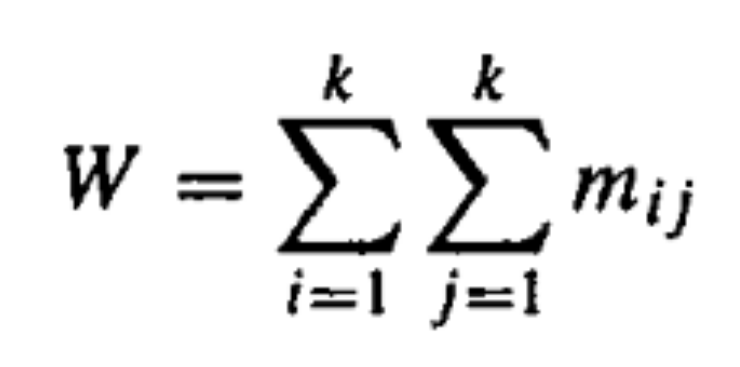
\includegraphics[width=0.25\textwidth]{imagenes/wsum} 
	\caption{Definición de W \cite{ref14}}
\end{figure}

Sabemos que, como mucho, ($k^2$ - k) entradas de M pueden ser etiquetadas como no monotónicas, por tanto el índice de no-monotonicidad queda así:

\begin{figure}[H]
	\centering
	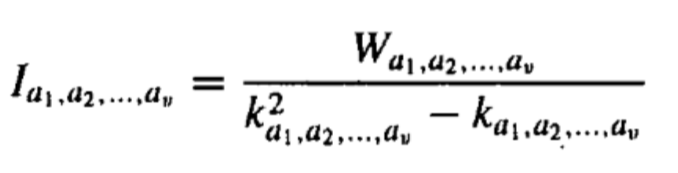
\includegraphics[width=0.5\textwidth]{imagenes/inm} 
	\caption{Definición índice de no-monotonicidad \cite{ref14}}
\end{figure}

Previo cálculo del índice que nos dirá como de bueno es un árbol tanto en precisión como en aguardar las restricciones monotónicas, calculamos el \textbf{order-ambiguity-score}, que se define en términos del índice previamente calculado tal como sigue:

\begin{figure}[H]
	\centering
	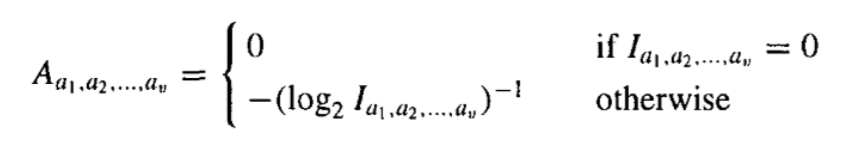
\includegraphics[width=0.75\textwidth]{imagenes/oas} 
	\caption{Definición de order-ambiguity-score \cite{ref14}}
\end{figure}

Finalmente, añadimos esta medida de no-monotonicidad calculada a nuestra medida de precisión E-score de la siguiente manera:

\begin{figure}[H]
	\centering
	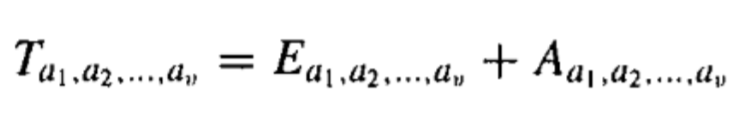
\includegraphics[width=0.55\textwidth]{imagenes/tas} 
	\caption{Definición de total-ambiguity-score \cite{ref14}}
\end{figure}

Una vez tenemos creada la métrica, ya sabemos que, a menor valor, mejor será el resultado, ya que significará que poseemos un menor fallo en la predicción y una mayor conservación de las relaciones de montonía dentro del árbol.

Esta forma de evaluar un árbol de decisión no implica que las consideraciones de monotonía deban dominar la construcción del árbol necesariamente. Podemos decidir cuánta importancia darle al proceso de construcción de un árbol montónico multiplicando el order-ambiguity-score por un factor para darle menor importancia al hecho de que el árbol aguarde las restricciones monotónicas con respecto al de que consiga una buena precisión en la predicción. \cite{ref14}

\newpage


